% !TeX document-id = {5f9589b8-498a-4233-98c1-605de3ca7afa}
% !TeX TXS-program:compile = txs:///pdflatex/[--shell-escape]


\documentclass[12pt, paper=a4, bibtotoc, toc=listof, headsepline=true]{scrreprt}

\usepackage[a4paper, includeheadfoot, %bindingoffset=3cm, 
left=2.75cm, right=2.75cm, top=2.5cm, bottom=3cm, headsep=0.8cm]{geometry}

%Header
\usepackage[automark]{scrpage2}
\pagestyle{scrheadings}
\clearscrheadfoot
\ohead{\rightmark}
\cfoot[\pagemark]{\pagemark}
\renewcommand*{\chaptermarkformat}{}
\renewcommand*{\headfont}{\normalfont}


%\setlength{\headheight}{12mm} % Höhe der Kopfzeile 




\setheadsepline[text]{0.4pt} % Trennlinie unter Kopfzeile 
%Abstand nach Header Trennlinie
%\usepackage[headsep=5mm]{geometry}

%\setfootsepline[text]{0.4pt} % Trennlinie unter Fußzeile






\setcounter{tocdepth}{3}% Include \subsubsection in ToC
\setcounter{secnumdepth}{3}% Number \subsubsection
\setuptoc{toc}{} % Adds ToC to ToC toDo: remove Pagenumber of ToC in ToC

\usepackage[ngerman]{babel} %Deutsch

\usepackage[utf8]{inputenc} %UTF8 Formatierung

\usepackage[T1]{fontenc}

\usepackage{helvet} %Arial
\renewcommand{\familydefault}{\sfdefault} %Arial

\usepackage{float}
\newfloat{listing}{tbhp}{lst}%[section]
\floatname{listing}{Listing}
\newcommand{\listoflistings}{\listof{listing}{Listing Verzeichnis}}

\usepackage{chngcntr}% http://ctan.org/pkg/chngcntr
\counterwithin{listing}{chapter} %counts chapters of listing




\usepackage[chapter]{minted} %Code Formatierung
\newminted{JavaScript}{frame=single,framesep=10pt, linenos, breaklines=true}
\newminted{HTML}{frame=single,framesep=10pt, linenos, breaklines=true}
\newminted{CSS}{frame=single,framesep=10pt, linenos, breaklines=true}

\usepackage{caption}
\DeclareCaptionFont{black}{\footnotesize\color{black}}
\DeclareCaptionFormat{listing}{{\parbox{\linewidth-2\fboxsep}{#1#2#3}}}
\setkomafont{captionlabel}{\usekomafont{caption}}




%Caption Listing, Figure Styling
\captionsetup[listing]{labelfont=black,textfont=black} %Caption of Listing
\captionsetup[figure]{labelfont=black,textfont=black} %Caption of Figure

\usepackage{graphicx} %IMG

\usepackage{csquotes}

\usepackage[onehalfspacing]{setspace} %Zeilenabstand


%\usepackage{apacite}
%\bibliographystyle{apacite} 
%%http://www.ctan.org/tex-archive/biblio/bibtex/contrib/apacite/apacite.pdf 
%\bibliography{library} % database is "thesis.bib" located in a "bibtex" subfolder 



\usepackage[
	backend=biber,
	style=numeric,
	sorting=none,
	language=german,
	urldate=comp,
	doi=false
]{biblatex}

\DefineBibliographyStrings{german}{%
	andothers = {et al.},
	and = {\&},
}
\DeclareFieldFormat{url}{\url{#1}}

\usepackage{url}
%\usepackage[draft=false]{hyperref}
\PassOptionsToPackage{hyphens}{url}

\usepackage[anythingbreaks]{breakurl}

\urlstyle{same}

\DeclareNameAlias{}{last-first} %Name in Literaturverzeichnis umdrehen
\DeclareBibliographyDriver{book}{%
	\printnames{author}%
	\setunit*{\addperiod\addspace}%
	\printfield[parens]{year}%
	\setunit*{\addperiod\addspace}%
	\printfield{title}%
	\setunit*{\addperiod\addspace}%
	\printlist{publisher}%
	\setunit*{\addperiod\addspace}%
	\printlist{location}%
	\finentry}

\DeclareBibliographyDriver{misc}{%
	\printnames{author}%
	\setunit*{\addperiod\addspace}%
	\printfield[parens]{year}%
	\setunit*{\addperiod\addspace}%
	\printfield{title}%
	\setunit*{\addperiod\addspace}%
	\printtext{Abgerufen am}
	\printfield{urlday}%
	\setunit*{\addperiod}%
	\printfield{urlmonth}%
	\setunit*{\addperiod}%
	\printfield{urlyear}%
	\setunit*{\newline}%
	\printtext{Abgerufen von}
	\printfield{url}%
	\finentry}

\AtEveryBibitem{
	
	%	\clearname{translator}%
	%	\clearlist{publisher}%
	\clearfield{isbn} %isbn ausblenden
	\clearfield{doi} %doi ausblenden	
	
}
\addbibresource{library.bib}

%Abkürzungen
\usepackage{acronym}

% Neues cite-Kommando oder altes \footcite-Kommando überschreiben
%\DeclareCiteCommand{\smfootcite}[\mkbibfootnote]
%{\usebibmacro{prenote}}                                 
%{\usebibmacro{citeindex}%
%	\setunit{\addnbspace}
%	\printnames{labelname}%
%	\setunit{\labelnamepunct}
%	\newunit
%	\printfield{year}
%}
%{\addsemicolon\space}
%{\usebibmacro{postnote}}


%\renewcommand{\smfootcite}[2][2]{\relax}



\pagenumbering{Roman} % Switch Roman

\title{Konzeption und Entwicklung von adaptiven Web Components}
\author{Christoph Kleber}
\date{\today}

\begin{document}

\maketitle

\chapter*{Kurzfassung}
\addcontentsline{toc}{chapter}{Kurzfassung}
In dieser Arbeit geht es um Web Components...
	
\chapter*{Abstract}
\addcontentsline{toc}{chapter}{Abstract}
This thesis is about Web Components...

\listoflistings
\listoffigures

\chapter*{Abkürzungsverzeichnis}
\addcontentsline{toc}{chapter}{Abkürzungsverzeichnis}
\begin{acronym}
	\acro{API}{Advanced Programming Interface}
	\acro{DOM}[DOM]{Document Object Model}
	\acro{HTML}[HTML]{Hypertext Markup Language}
	\acro{URL}[URL]{Uniform Resource Locator}
	\acro{HTML5}[HTML5]{Hypertext Markup Language Version 5}
	\acro{CSS}[CSS]{Cascading Style Sheets}
	\acro{W3C}{World Wide Web Consortium}
	\acro{REST}{Representational State Transfer}
	\acro{HTTP}{Hypertext Transfer Protocol}
	\acro{JSON}{JavaScript Object Notation}
	\acro{WCAG 2.0}{Web Content Accessibility Guidelines 2.0}
	\acro{AWC Framework}{Adaptive Web Components Framework}
\end{acronym}

\tableofcontents




\chapter{Adaptivität}
\pagenumbering{arabic} % Switch to normal numbers
Der Begriff Adaptivität wird in vielen verschiedenen Kontexten genutzt. Die Bedeutung ist somit mehrdeutig und abhängig vom Umfeld. Beispielsweise wird in der Psychotherapie unter Adaptivität im therapeutischen Vorgehen eine \enquote{Grundhaltung [beschrieben], welche die Bereitschaft impliziert, unter stetiger Reflexion der Prozesse von Übertragung und Gegenübertragung flexibel auf die jeweils aktuellen Bedürfnisse des Patienten einzugehen}\cite[S. 45]{woeller2014tiefenpsychologisch}. Im Kontext von Datenbanken und der \enquote{Adaptivität an unterschiedliche Anforderungen} wird von Verfahren gesprochen, die \enquote{die Anpassungsfähigkeit an unterschiedliche Anforderungen und damit auch an verschiedene Einsatzumgebungen [erhöhen]}\cite[][S. 112]{loeser2013web}.
In der Softwareentwicklung kann Adaptivität folgendermaßen beschrieben werden: \enquote{Interaktive Softwaresysteme werden von Benutzern mit unterschiedlichsten Zielen, Interessen, Fähigkeiten, Erfahrenheitsgraden und Präferenzen verwendet. Um einem möglichst breitem Personenkreis zugänglich zu sein, bieten viele derzeit erhältliche Programme bereits die Möglichkeit, daß Benutzer (oder Systemadministratoren) in bestimmtem Ausmaß eine Anpassung des Programms an die jeweiligen individuellen Präferenzen vornehmen können}\cite[S. 1]{Kobsa1993}.
\newline In den verschiedenen Auslegungen des Wortes ist ein Muster zu erkennen. Adaptivität kann definiert werden als die Fähigkeit eines Objekts, zum Beispiel eine Person oder ein System, sich an seine Umgebung anzupassen. Diese Anpassung basiert auf bestimmten Einflüssen, so kann sich eine Datenbank an äußere Einflüsse, wie beispielsweise ihre Einsatzumgebung, oder ein Softwaresystem an die Vorlieben seines Nutzers anpassen. Das kann auch automatisch geschehen. So gleicht sich beispielsweise der Inhalt der Seite \enquote{Facebook} aufgrund eines Algorithmus an den einzelnen Nutzer an, ohne dass dieser bestimmte Einstellungen vornehmen muss\cite{Rixecker2016}. Die Möglichkeit zur Adaptivität kann jedoch auch dem Nutzer bereitgestellt werden. Ist das der Fall, kann der Nutzer beispielsweise die Benutzeroberfläche nach seinen eigenen Vorlieben einrichten. So kann zum Beispiel die Benutzeroberfläche der Entwicklungsumgebung \enquote{JetBrains PhpStorm} anhand persönlicher Präferenzen aufgebaut werden und Farbstile und Kontraste verändert werden.
\newline Hier stellt sich jedoch die Frage, wie im Zusammenhang von Internetanwendungen eine Adaptivität bereitgestellt werden kann und insbesondere, an welche Aspekte sie sich adaptieren soll. Hierfür muss die Umgebung, der Nutzer und auch dessen Arbeitsaufgaben erforscht und definiert werden.
	\section{Nutzungskontext}
	Die Betrachtung des Nutzungskontext bietet diese Möglichkeit. Der Nutzungskontext wird nach der DIN EN ISO 9241-210 von den Benutzermerkmalen, Arbeitsaufgaben und der organisatorischen, technischen und physischen Umgebung bestimmt. Im Folgenden wird ein Überblick dieser Beschreibung gegeben\cite[S.15 ff.]{hoffmann2014venus}.
	\begin{description}  
		\item  [Nutzer und sonstige Interessengruppen] 
		Zu Beginn sollten die Nutzergruppen und weitere Interessengruppen identifiziert und deren wesentliche Ziele und Einschränkungen beschrieben werden.
			
		\item [Merkmale der Nutzer oder Nutzergruppen]
		Diese Merkmale können \enquote{Kenntnisse, Fertigkeiten, Erfahrung, Ausbildung, Übung, physische Merkmale, Gewohnheiten, Vorlieben und Fähigkeiten einschließen}\cite[S.16 ]{hoffmann2014venus}. Sie beschreiben also insgesamt den Nutzer, um diesen besser einordnen und sich besser an diesen anpassen zu können.
		
		\item  [Ziele und Arbeitsaufgaben der Nutzer]
		Auf der einen Seite werden die Ziele der Nutzer beschrieben, auf der anderen Seite die Gesamtziele des Systems. Danach müssen die Arbeitsaufgaben betrachtet und nach ihren Merkmalen untersucht werden, beispielsweise wie oft eine Aufgabe ausgeführt werden soll.
			
		\item [Umgebung(en) des Systems]
		Die Umgebung lässt sich in die technische Umgebung, also die der Computerkomponenten und Anwendungen, die physikalische Umgebung, also Aspekte wie beispielsweise Beleuchtung und soziale und kulturelle Umgebung aufteilen. Zur kulturellen Umgebung zählen beispielsweise die Arbeitsweise und Einstellungen der Umgebung des Systems.
	\end{description}
	Insgesamt lässt sich somit sagen, dass die Adaptivität an den Nutzungskontext ausgerichtet werden kann. Verschiedene Merkmale des Nutzungskontext haben Einfluss darauf, wie die Adaptivität, passend zur Situation, erfolgen sollte.
		
\chapter{Web Components}
	\emph{Web Components} sind eine \ac{W3C} Spezifikation. Diese soll es ermöglichen, eigenständige und wiederverwertbare Komponenten für Web Anwendungen zu erstellen\cite[S. 1]{patel2015learning}. Sie setzen sich zusammen aus den vier Technologien \emph{Custom Elements}, \emph{\ac{HTML} Imports}, \emph{Templates} und \emph{Shadow \ac{DOM}}. Das Nutzen dieser Technologie soll Applikationen im Web leichter wiederverwertbar, wartbar, unabhängiger und kapselbar machen\cite[S.2]{patel2015learning}.
	\section{Geschichte der Web Components}
	\label{ref:gesVonWebCom}
	\emph{Web Components} wurden vom \ac{W3C} das erste Mal im Jahr 2012 als ein \emph{Working Draft}, also Arbeitsentwurf, erwähnt. Hier wurde es auch \emph{Component model for the web} genannt und bestand aus den vier Technologien \emph{Templates}, \emph{Decorators}, \emph{Custom Elements} und \emph{Shadow DOM}. In der derzeitigen Version der \emph{Web Components} wird die \emph{Decorators} Technologie nicht mehr verwendet. Die \emph{\ac{HTML} Import} Technologie wurde jedoch zu den \emph{Web Components} ergänzt\cite{Cooney2012}. Da die \emph{Web Components} aus verschiedenen Technologien zusammengesetzt sind, wird in dem nächsten Abschnitt auf die Geschichte der einzelnen Technologien eingegangen um einen Überblick zu verschaffen. Hierbei wird insbesondere auf die erste Unterstützung der Technologien in den verschiedenen Browsern und die heutige Browserkompatibilität eingegangen.
		\subsection{Custom Elements}
		\emph{Custom Elements} liegen in der Version v0 und in der Version v1 vor. Die Version v0 wurde das erste Mal im Jahr 2014 von den Browsern \emph{Chrome} in der Version 33 und \emph{Opera} in der Version 20 unterstützt. In den mobilen Varianten dieser Browser  wird sie seit 2016 von \emph{Opera for Android} in der Version 37 und von \emph{Chrome for Android} in der Version 53 verwendet\cite{C2015}. Im \emph{Android} Browser ist diese Version schon seit 2014 in Gebrauch, in der \emph{Android} Version 4.4.4. Im \emph{Samsung Internet} wird sie seit 2016 in der Version 4 genutzt\cite{cusEleCanIUse}. Die Version v0 wird von der Version v1 abgelöst, hier ergeben sich einige Änderungen in der Syntax der \ac{API}\cite{Bidelman2016cusElev1}. Derzeit wird sie nicht per Standardeinstellung von anderen Browsern unterstützt\cite{firefox}, im Gegensatz zur Version v1. \emph{Chrome} und \emph{Opera} unterstützen diese. Das erste mal wurde sie im Jahr 2016 in der \emph{Chrome} Version 54 und in der \emph{Opera} Version 41 genutzt\cite{C2016}.
		\subsection{HTML Imports}
		\emph{\ac{HTML} Imports} wurden in den Browsern \emph{Chrome} und \emph{Opera} zuerst 2014 verwendet. Die \emph{Imports} wurden als Erstes in der \emph{Chrome} Version 36 und in der \emph{Opera} Version 23 genutzt. Gegenwärtig wird die Technologie von den zuvor erwähnten Browsern auch in den mobilen Browser-Varianten unterstützt, in den Versionen 53 des \emph{Chromium} und 37 des \emph{Opera for Android}\cite{Morrita2015}. Der \emph{Android} Browser hat die  \emph{\ac{HTML} Imports} seit 2016 in Gebrauch, in der Version 53. Der Browser des \emph{Android} Betriebssystems ist ab dem Jahr 2016 in der Version 53 kongruent mit dem Chromium Browser. \emph{Samsung Internet} unterstützt die \emph{Imports} seit 2016 in der Version 4\cite{htmlTemplCaniuse}.
		\subsection{Decorators}
		\emph{Decorators} erscheinen nur in Dokumenten und Artikeln, sie wurden nie von Browsern implementiert. So wird im Jahr 2012 in einem \emph{Working Draft} des \ac{W3C} von einem Beispiel gesprochen: \enquote{Here is an example of how decorators could be used to implement a simple variant of the details element}\cite{Cooney2012}. Dies zeigt, dass an dieser Stelle noch keine Implementierung der Technologie vorliegt. Auch in einem Arbeitsentwurf des \ac{W3C} vom Jahr 2013 wird davon gesprochen, dass \enquote{Decorators, unlike other parts of Web Components, do not have a specification yet}\cite{Cooney2013}.
		Auf einer aktuellen Übersichtsseite des Konsortiums wird die \emph{Decorators} Technologie nicht mehr im Zusammenhang mit \emph{Web Components} erwähnt\cite{WebComCur2016}.
		\subsection{Templates}
		\emph{Templates} werden schon über einen längeren Zeitraum in den verschiedenen Browsern unterstützt. Zuallererst wurden sie im \emph{Chrome} im Jahr 2013 verwendet, in der Version 26. Im selben Jahr wurden sie vom \emph{Firefox} Browser in der Version 22 und vom \emph{Opera} Browser in der Version 15 erstmals verwendet\cite{W2015}\cite{htmlTemFire}.
		Im Jahr 2015 wurden sie dann vom \emph{Edge} Browser unterstützt, in der Version 13\cite{build10547}.
		Auf den Browsern des \emph{Macintosh} Betriebssystems wurden \emph{Templates} zuerst 2014 verwendet, in der \emph{Safari} Version 7.1 und der \emph{Safari \& Chrome for iOS} Version 8\cite{htmlTemplCaniuse}. In den meisten mobilen Varianten der Browser werden \emph{Templates} seit 2016 bereitgestellt. So erschien diese Funktion in dem \emph{Opera for Android} Browser in der Version 37, in \emph{Chrome for Android} in 53, in \emph{Firefox for Android} in 49 und im \emph{Samsung Internet} Browser in der Version 4. Der Standard Android Browser unterstützt \emph{Templates} jedoch schon seit 2013, in der Version 4.4\cite{htmlTemplCaniuse}.
		\subsection{Shadow DOM}
		Der \emph{Shadow \ac{DOM}} existiert in der Version v0 und in der Version v1. Die Version v0 wird seit 2014 vom \emph{Chrome} in der Version 35 und \emph{Opera} Browser in der Version 21 unterstützt. Mit der Safari Version 10 kann der \emph{Shadom \ac{DOM}} seit 2016  genutzt werden\cite{NiwaShaDom}. Die mobilen Varianten der Browser gebrauchen das \emph{Shadow \ac{DOM}} seit 2016, \emph{Opera} in der Version 37 und \emph{Chrome} in der Version 53, somit auch der \emph{Android} Browser\cite{Hayato2016}. Die Version v0 wird von der Version v1 abgelöst, welche verschiedene Neuerungen in der Syntax, aber auch in dem Gebrauch von bestimmten Funktionen aufweist. So kann beispielsweise in der v0 ein \emph{shadow root} immer nur als \enquote{open} definiert werden, in der v1 kann er auch als \enquote{closed} \emph{shadow root} erstellt werden\cite{Ito2016}.
		Die Version v1 wird noch nicht in so großem Ausmaß wie die Version v0 unterstützt. Vollständig wird sie nur vom \emph{Chrome} 53 und \emph{Opera} 40 Browser genutzt, jeweils seit 2016. In den mobilen Versionen wird sie nur von dem \emph{Chromium} und somit auch auf \emph{Android} in der Version 53 verwendet\cite{Hayato2016a}.
	
			
	\section{Technik der Web Components}
	Im Folgenden werden die technischen Grundlagen der \emph{Web Components} und insbesondere deren Syntax erforscht und durch Beispiele erläutert.
		\subsection{Custom Elements}
		Das \emph{Custom Element} ist eine \ac{API}, welches das Bilden eigener, voll funktionstüchtiger \ac{DOM} Elemente ermöglicht\cite{Denicola2016}. Die \ac{API} beschreibt in diesem Zusammenhang eine Schnittstelle, die einem anderen Programm ein Werkzeug zur Verfügung stellt, um sich an das eigene Softwaresystem anbinden zu können\cite{Behrendt2016}. Somit ermöglicht eine \ac{API} einen Austausch von Informationen zwischen verschiedenen Programmen oder Systemen.	
		Die \emph{Custom Element} \ac{API} ermöglicht den Nutzern die Auszeichnungsprache \ac{HTML} zu erweitern\cite{Argelius2016}. Es können bestehende \ac{HTML} Elemente erweitert, oder neue hinzugefügt werden. Jedes neue oder erweiterte Element wird unter einem \emph{Tag} Namen registriert. Dies ermöglicht eine Kapselung des erstellen Programmiercodes in Elemente. In Listing \ref{lst:cusEleJav} ist ein JavaScript Programmcode dargestellt, der ein leeres \emph{Custom Element} definiert und unter dem Namen \enquote{new-custom-element} registriert wird.
		\begin{listing}
			\begin{JavaScriptcode*}{}
class NewCustomElement extends HTMLElement { //Definition custom element
	constructor() {
		super();
	}
}
customElements.define('new-custom-element', NewCustomElement); //Registrierung custom element
			\end{JavaScriptcode*}
			\caption{Custom Element JavaScript}
			\label{lst:cusEleJav}
		\end{listing}
		Für \emph{Custom Elements} sind mehrere \emph{Callbacks} verfügbar. \emph{Callback} Funktionen beschreiben hier Funktionen, die bei bestimmten Ereignissen des Lebenskreislaufs der Applikation von außerhalb des \emph{Custom Elements} aufgerufen werden. Im Folgenden werden diese Funktionen aufgelistet\cite{Argelius2016}.
		\begin{description}  
			\item  [\emph{connectedCallback()}] Diese Funktion wird aufgerufen, wenn das \emph{Custom Element} an den \ac{DOM} angehängt wird.			
			\item [\emph{disconnectedCallback()}] Diese Funktion wird aufgerufen, wenn das \emph{Custom Element} vom \ac{DOM} wieder losgelöst wird. 			
			\item  [\emph{attributeChangedCallback(name, prevValue, newValue)}] Diese Funktion wird aufgerufen, wenn sich ein Attribut ändert; jedoch nur für Attribute aufgerufen, die in einer statischen \emph{get} Funktion mit Namen \emph{observedAttributes} definiert wurden.
		\end{description}
		\subsection{HTML Imports}
		\emph{\ac{HTML} Imports} ist eine Technologie zum Importieren von externen \ac{HTML} Dokumenten in ein \ac{HTML} Dokument. Hier unterscheidet man zwischen importierenden und importierten \ac{HTML} Dokumenten. Die importierenden Dokumente besitzen einen Link, der mindestens die \ac{URL} des \emph{Imports} und die Eigenschaft \emph{rel=\enquote{import}} besitzt,also ein Link eines bestimmten Typ ist\cite{Glazkov2016}.(siehe Listing \ref{lst:htmImp}) 
		\begin{listing}
			\begin{HTMLcode*}{}
 <link rel='import' href='/imports/imported-document.html'>
				\end{HTMLcode*}
			\caption{Standard HTML Import}
			\label{lst:htmImp}
		\end{listing}
		Die importierten Dokumente haben keinen außergewöhnlichen Aufbau im Vergleich zu normalen \ac{HTML} Dokumenten, sie können aus \ac{HTML}, \ac{CSS} oder JavaScript Elementen bestehen. Es kann auch die \emph{Template} Technologie verwendet werden, dazu mehr in Kapitel \ref{subsec:Templates}.
		Um auf den Inhalt des importierten Dokuments zuzugreifen wird JavaScript verwendet. Wie in Listing \ref{lst:htmImpJav} dargestellt, wird zuerst nach dem Link Element gesucht, welches die Eigenschaft rel=\enquote{import} besitzt. Daraufhin wird dieses Dokument importiert und ein bestimmter Teil des Dokuments als JavaScript Variable \enquote{elem} gespeichert. Hier wird ein div Element, das mit der Klasse \enquote{element} ausgezeichnet ist, gespeichert. Anschließend kann dies in der importierenden Seite genutzt werden. 
		\begin{listing}
			\begin{JavaScriptcode*}{}
var link = document.querySelector('link[rel=import]'); //durchsucht nach zu importierendem Link
var importedDocument = link.import; //importiert den Inhalt des Links
var elem = importedDocument.querySelector('div.element');  //Selektiert Element der importierten Komponente
			\end{JavaScriptcode*}
			\caption[Zugriff auf importiertes Dokument]{JavaScript Programmcode für Zugriff auf Inhalt des importierten Dokuments}
			\label{lst:htmImpJav}
		\end{listing} 
		\subsection{Templates}
		\label{subsec:Templates}
		Das \ac{HTML5} Feature \emph{Template} ermöglicht Teile einer Seite unabhängig vom \ac{DOM} zu erstellen. Diese können dann später programmatisch zum \ac{DOM} hinzugefügt werden\cite[S.177]{Cameron2015}. Das bedeutet, dass der Inhalt des \emph{Templates}, bis er zum \ac{DOM} hinzugefügt wird, nicht in der Webanwendung angezeigt wird und auch nicht über \ac{DOM} Selektoren angesteuert werden kann. Gegebenenfalls im \emph{Template} enthaltene Bilder werden nicht geladen und Skripte nicht ausgeführt\cite{Potschien2013}.
		\begin{listing}
			\begin{JavaScriptcode*}{}
var inhalt = document.querySelector('template').content;
document.querySelector('body').appendChild(inhalt);
			\end{JavaScriptcode*}
			\caption[Hinzufügen eines Templates]{JavaScript Programmcode für das Hinzufügen eines Templates in das DOM}
			\label{lst:htmTem}
		\end{listing}
		In Listing \ref{lst:htmTem} sieht man den JavaScript Programmcode um ein vorhandenes \emph{Template} zum \ac{DOM} hinzuzufügen. In Zeile eins wird der Inhalt des \emph{Templates} zur JavaScript Variable \enquote{inhalt} hinzugefügt, um dann in der nächsten Zeile an den \emph{body} der Seite, also dem eigentlichen Inhalt hinzugefügt zu werden. In diesem Moment werden ebenso die Bilder des \emph{Templates} geladen und eventuelle Skripte ausgeführt.
		\subsection{Shadow DOM}
		\enquote{Das \emph{Shadow \ac{DOM}} beschreibt die Fähigkeit eines Browsers, eine neue, völlig ab gekapselte Knotenstruktur im bestehenden \ac{DOM} zu erzeugen}\cite[Kap. 11.1.4]{gasston2014moderne}. Dies bedeutet, dass neben dem normalen \emph{Document tree}, dessen Wurzelknoten ein Dokument ist, noch der \emph{Shadow tree} besteht. Der Wurzelknoten des letzteren ist kein Dokument, sondern der \emph{Shadow root}.
		\iffalse
			Dies ist in Abbildung \ref{img:shaDom} dargestellt\cite[S.22]{patel2015learning}.
			\begin{figure}
			\centering
			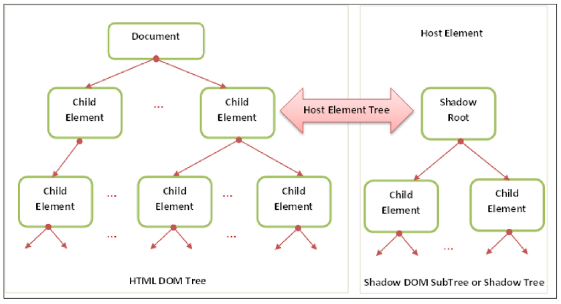
\includegraphics[width=\textwidth,height=\textheight,keepaspectratio]{shaDom.png}
			\caption{DOM und Shadow DOM\cite[S. 22]{patel2015learning}}
			\label{img:shaDom}
			\end{figure}
		\fi
		Die Folge dieser Kapselung ist, dass alles was dem \emph{Shadow tree} hinzugefügt wird, nur lokal Einfluss hat. Die Gestaltung von Webelementen im \emph{Shadow root} wird dadurch vereinfacht.
		\ac{CSS} Selektoren können dadurch nicht von außerhalb des \emph{Shadow roots} auf diesen zugreifen und Selektoren, die innerhalb dieses definiert werden haben keinen Einfluss auf den normalen \ac{DOM}. Genauso verhält es sich mit dem Zugriff auf die \ac{DOM} Elemente des \emph{Shadow root}. Sie können nicht von außerhalb angesprochen werden, beispielsweise durch die Funktion \enquote{document.querySelector()}, sondern können nur von Funktionen innerhalb des \emph{Shadow root} angesprochen werden\cite{Bidelman2016}.
		\begin{listing}
			\begin{JavaScriptcode*}{}
var header = document.createElement('header'); 
var shadowRoot = header.attachShadow({mode: 'open'}); //shadow root an header angefügt
var headline = document.createElement('h1'); 
var headlineText = document.createTextNode('headline');
headline.appendChild(headlineText);
shadowRoot.appendChild(headline); //Elemente als Kinder in shadow root angefügt
			\end{JavaScriptcode*}
				\caption[Erstellung eines Shadow DOM]{JavaScript Programmcode für die Erstellung eines Shadow DOM}
				\label{lst:javShaDom}
		\end{listing}
		In Listing \ref{lst:javShaDom} ist dargestellt, wie Mithilfe von JavaScript ein \emph{Shadow \ac{DOM}} erstellt wird. In Zeile zwei wird zuerst einem bestehendem Element ein \emph{Shadow root} hinzugefügt. Daraufhin wird eine Überschrift und deren Text erstellt und zusammengefügt. Zuletzt wird in Zeile sechs die Überschrift in den \emph{Shadow \ac{DOM}} eingefügt.
			\subsubsection{Slots}
			\emph{Shadow \ac{DOM}} kann auch mit anderen \ac{DOM} erweitert werden. Der Entwickler kann dem Nutzer seines \emph{Web Component} ermöglichen, diesen zu erweitern. Hierfür werden \emph{Slots} verwendet. 
			\begin{listing}
				\begin{HTMLcode*}{}
<ul id='contacts'>
   <li>
      <slot name='title'>Kein Titel</slot> <!-- Slot Element title mit Platzhalter 'Kein Titel' -->
      <slot name='name'> <!-- Slot Element mit Platzhalter -->
         <p>Achtung<p>
         <h1>Kein Name<h1>
      </slot>
   </li>
</ul>
				\end{HTMLcode*}
				\caption[Slot Elemente im Shadow DOM]{Nutzung von Slot Platzhalter-Elementen im Shadow DOM}
				\label{lst:sloNutShaDom}
			\end{listing}
			In Listing \ref{lst:sloNutShaDom} ist der \ac{HTML} Programmcode des \emph{Web Component} dargestellt, welcher im \emph{Shadow \ac{DOM}} später gerendert wird. Hier ist die Verwendung des \emph{Slot} Elements interessant. Dieses kann beim Einbinden des \emph{Web Component} später ausgestattet werden. Wird das Platzhalter-Element später nicht befüllt, wird das \emph{Fallback}, also die Ersatzfunktion, der Inhalt innerhalb des Elements, hier beispielsweise \enquote{Kein Titel} genutzt. Die Ersatzfunktion kann auch aus einem eigenen \ac{DOM} Baum bestehen, wie im \emph{Slot} \enquote{name} zu sehen ist\cite{Bidelman2016}. In Listing \ref{lst:sloNutLigDom} werden die, in Listing \ref{lst:sloNutShaDom} erstellten Platzhalter-Elemente, beim Verwenden des \emph{Web Component} in beispielsweise einer Webseite befüllt. Wie hier in Zeile fünf und sechs zu sehen ist, können einzelne Slots auch mit mehreren Elementen befüllt werden. Beim Übersetzen des Programmcodes der Applikation werden alle Elemente, die die passenden \emph{Slot} Attribute aufweisen in den \ac{DOM} übersetzt. Wenn im \emph{Shadow \ac{DOM}} ein \emph{Slot} Platzhalter ohne ein \enquote{name} Attribut definiert wird, werden alle vom Nutzer innerhalb des \emph{Web Components} erstellten Elemente in den \emph{DOM} geschrieben.
			\begin{listing}
				\begin{HTMLcode*}{}
<span slot='title'>Dr.</span> <!-- Element mit Slot Attribut -->
<span slot='title'>Phil.</span> <!-- Element mit Slot Attribut -->
<span slot='name'>Michael</span> <!-- Element mit Slot Attribut -->
				\end{HTMLcode*}
				\caption{Befüllen der Slot Elemente im DOM}
				\label{lst:sloNutLigDom}
			\end{listing}
			In Listing \ref{lst:renDom} ist der von den zwei vorhergehenden Listings kombinierte und gerenderte Inhalt zu sehen. Dies ist der \ac{DOM}, den man beispielsweise in einer Webseite sehen würde. Hier ist gut zu erkennen, wie die \emph{Slot} Elemente des \emph{Shadow \ac{DOM}} mit den später erstellten Elementen befüllt werden. Alle Elemente innerhalb des \emph{Web Component} mit dem Attribut \enquote{slot} werden in diesen übertragen.
			\begin{listing}
				\begin{HTMLcode*}{}
<ul id='contacts'>
   <li>
      <slot name='title'> <!-- Übersetztes Slot Element title -->
	     <span>Dr.</span>
	     <span>Phil.</span>
	  </slot>
      <slot name='name'> <!-- Übersetztes Slot Element name -->
	     <span>Michael</span>
      </slot>
   </li>
</ul>
				\end{HTMLcode*}
				\caption{Übersetzter DOM}
				\label{lst:renDom}
			\end{listing}
		\subsubsection{Shadow DOM Stil-Regeln}
		Wie auf den vorherigen Seiten erklärt, ist der \emph{Shadow tree} vom normalen \ac{DOM} abgekapselt. Dies hat zur Folge das \ac{CSS} Stil-Regeln, definiert im eigenen \emph{Component}, nur Einfluss auf den \emph{Shadow tree} des \emph{Web Component} haben. Es können \ac{CSS} Selektoren verwendet, die auch außerhalb des Element bestehen. Trotzdem haben diese keinen Einfluss auf außerhalb. \newline
		Eine Besonderheit der Stil-Regeln des \emph{Shadow DOM} sind dessen Selektoren. Der \enquote{:host} Selektor definiert den Stil für das Element, in welchem der \emph{shadow tree} bereitgestellt wird, somit für den \emph{Web Component}. Dieser wirkt nur in dem Kontext eines \emph{shadow root}. Dadurch kann der Stil des eigenen \emph{Web Component} verändert werden. Eine Eigenschaft des \enquote{:host} Selektors ist, dass die Seite, welche das \emph{Web Component} enthält, stärkeren Einfluss auf diesen Selektor besitzt und somit den Stil überschreiben kann. Damit ermöglicht es den Nutzern eines \emph{Web Component}, diesen nach eigenen Wünschen anzupassen. Darüber hinaus kann der \enquote{:host} Selektor erweitert werden. So können über die Form \enquote{:host(<selector>)} bestimmte Stil Eigenschaften gesetzt werden, welche nur Anwendung finden wenn das \emph{Web Component} bestimmte Eigenschaften erfüllt. 
		\begin{listing}
		\begin{HTMLcode*}{}
<style>		
:host(:hover) { /* :host Selektor bei hover Zustand */
   opacity: 1;
}
:host(.blue) { /* :host Selektor bei Vorhandensein der Klasse blue */
   color: blue;
}
</style>
		\end{HTMLcode*}
		\caption{Der :host Selektor}
		\label{lst:hosSel}
		\end{listing}
		In Listing \ref{lst:hosSel} ist dargestellt in welcher Form Einfluss genommen werden kann. So spricht der Selektor in Zeile zwei nur den \emph{Web Component} an, während die Maus sich über diesem befindet. Der Selektor in Zeile fünf spricht nur den \emph{Web Component} an, wenn dieser die Klasse \enquote{blue} erhalten hat.
		\section{Webentwicklung mithilfe der Web Components}
		Das \emph{Frontend} von modernen Webseiten basiert heutzutage hauptsächlich auf den Technologien \ac{HTML}, \ac{CSS} und JavaScript. Meistens werden darüber hinaus noch verschiedene \emph{Frameworks} verwendet. \enquote{A computer system framework has a layered structure that can incorporate servers, operating systems, client machines, and applications. The framework can provide a set of functions to definde application interfaces, the interrelationships between applications, and internal communications between clients and external to online platforms}\cite[S.15]{stuart2013roadmap}. Ein \emph{Framework} ist somit ein System, das den Entwicklern bestimmte Funktionalitäten zur Verfügung stellt, ohne dass dieser sie selbst programmieren muss. Sie können beispielsweise die Hilfe bei der Interaktion mit dem \ac{DOM} sein, wie das JavaScript \emph{Framework} \enquote{jQuery}, ein \enquote{Slide-Element} bereitstellen wie das \emph{Framework} \enquote{Slider} oder zur Diagrammerstellung genutzt werden wie das \emph{Framework} \enquote{D3}. Hier ergibt sich ein Problem. Wenn in einer Applikation mehrere \emph{Frameworks} und Technologien für verschiedene Funktionen verwendet werden, können sich diese gegenseitig beeinflussen. So können die Stil-Regeln verschiedener Teile der Webseite sich unbeabsichtigt beeinträchtigen oder das JavaScript, das eine bestimmte Funktion hat, an einer anderen Stelle für die es nicht programmiert wurde, Einfluss nehmen. Viele dieser Probleme resultieren daraus, dass verschiedene \emph{Frameworks} für Variablen oder Funktionen die gleiche Benennung nutzen und somit manche Elemente doppelt benannt und damit auch doppelt angesprochen werden. Darüber hinaus können viele Teile der Webseite weder wiederverwendet, noch gut gewartet werden, da sie großen Einfluss aufeinander nehmen und somit sehr ineinander verschachtelt sind.
		Die \emph{Web Components} versuchen diese Probleme durch eine (in Zukunft) native Implementierung verschiedener Techniken anzugehen, die eine Kapselung, eine Wiederverwendung und eine leichtere Wartbarkeit von Programmcode ermöglichen sollen. Nachfolgend wird auf die daraus resultierenden Vor- und Nachteile eingegangen. 			
			\subsection{Native Browserunterstützung}
			Aufgrund der Erkenntnisse der Geschichte von \emph{Web Components} in Kapitel \ref{ref:gesVonWebCom} ist eine gewisse Wahrscheinlichkeit gegeben, dass die Technologien der \emph{Web Components} in Zukunft nativ von den verschiedenen Browsern unterstützt werden.
			Sollte dieser Fall eintreffen ergibt sich daraus ein großer Vorteil. Es muss bei der Nutzung nativer, also von den Browsern implementierten Techniken, kein externer Programmcode genutzt werden um bestimmte Funktionen abzudecken. Viele Funktionalitäten können einfach über die Nutzung nativer Methoden abgebildet werden. Deshalb müssen weniger Funktionen selbst geschrieben und weniger, beziehungsweise unter Umständen keine \emph{Frameworks} genutzt werden. Dies verkleinert das Laden von externen Programmcode. Außerdem ist die Syntax und Funktionsweise bei nativen Funktionen bekannt und eindeutig. Daraus ergeben sich weniger Inkonsistenzen in der Programmierung und eine leichtere Verständlichkeit. Im Gegensatz dazu muss bei vielen \emph{Frameworks} eine jeweils eigene Syntax benutzt werden.
			\subsection{Kapselung}
			Ein Mechanismus zur Datenkapselung wird vom \emph{Shadow DOM} bereitgestellt.
			Dieser ermöglicht, dass der Programmcode des \emph{Web Components} vom Rest der Applikation getrennt werden kann. Dadurch wird ein privater \emph{Scope}, also ein Geltungsbereich der Applikation und dessen Variablen, Methoden und Bezeichnern, genutzt\cite[S.2]{patel2015learning}. Dies hat einige Folgen für das Verhalten einer Applikation. Zuerst ist der \emph{Shadow \ac{DOM}} isoliert. Er kann nicht von außerhalb angesprochen werden, beispielsweise über die Funktion \enquote{document.querySelector()}. Dies hat den Vorteil, dass die Funktionalität des \emph{Web Component} nicht von außen beeinträchtigt werden kann. Außerdem hat das \ac{CSS} nur Zugriff auf den \ac{DOM} des eigenen Geltungsbereichs; weder von außerhalb noch von innerhalb nach außen des \emph{Shadow \ac{DOM}} können Stil-Regeln Einfluss nehmen. Ein Vorteil an dieser Eigenschaft ist, dass man atomare, also sehr einfache, \ac{CSS} Bezeichner innerhalb des \emph{Shadow \ac{DOM}} verwenden und dieselben Bezeichner gleichzeitig außerhalb dieses nutzen kann\cite{Bidelman2016}. Darüber hinaus wird die Gestaltung der Erscheinung der Applikation beständiger. Sie erfolgt einzeln für jedes \emph{Web Component} und für den Bereich außerhalb der \emph{Web Components}.
			\subsection{Wiederverwendung}
			Die Theorie der \emph{Web Components} ist die Erstellung von verschiedenen Komponenten, die wiederverwendet werden können. Dies hat zum einen den großen Vorteil, dass es eine Interoperabilität zwischen \emph{Frameworks} ermöglicht\cite[S.2]{patel2015learning}. Dadurch ist man nicht an ein bestimmtes \emph{Framwork} gebunden und kann auch mit Elementen außerhalb dieses Ökosystems interagieren und Komponenten wiederverwenden. Zum anderen können auch innerhalb eines \emph{Frameworks} oder nativ, ohne das Nutzen eines \emph{Frameworks}, Teile der Anwendung wiederverwendet werden, was eine Arbeitserleichterung und Verminderung des Programmcodes hervorruft. 
			\subsection{Wartbarkeit}
			Die Wartbarkeit von Web-Applikationen wird erleichtert, da die \emph{Web Components} in \emph{Templates} organisiert sind\cite[S.2]{patel2015learning}. Das sorgt dafür, dass der Programmcode einzelner Komponenten separat gespeichert und somit leichter wiedergefunden und geändert werden kann.
			\subsection{Browserunterstützung}
			Auch wenn \emph{Web Components} sehr viele Vorteile aufweisen, ist es ein Problem wenn die Techniken (noch) nicht in allen Browsern unterstützt werden oder unterschiedlich implementiert sind. Wie in Kapitel \ref{ref:gesVonWebCom} dargelegt, werden einige der Techniken noch nicht von allen Browsern unterstützt oder unterscheiden sich in deren Umsetzung. Dies kann zu Inkonsistenzen oder dem nicht Funktionieren einer Applikation führen. Durch Verwendung von  \emph{Polyfills} kann man dies jedoch umgehen. Das sind in diesem Zusammenhang Programmcodes, die die Funktionen oder Teile einer Technologie, die nativ noch nicht von einem Browser unterstützt wird, nachstellen. Sie können dann verwendet werden um Nutzern aller Browser den Gebrauch der Technologien zu ermöglichen\cite[S.4]{satrom2014building}. Das \emph{webcomponents.js} ist ein Set von \emph{Polyfills} und ermöglicht den Nutzern die Verwendung von \emph{Web Components} in allen modernen Browsern\cite{webComJs}.
\chapter{Polymer}
Die \emph{Polymer} Bibliothek stellt eine Sammlung von Funktionen bereit um \emph{custom elements} zu erstellen. Diese Elemente sollen letztendlich wie normale \ac{DOM} Bestandteile funktionieren\cite{polymerFeaOve}.
	\section{Polymer Technologie} Die verwendeten Technologien der Bibliothek ähneln den \emph{Web Components} oder es werden direkt die Technologien der \emph{Web Components} genutzt. Im Folgenden wird die Technologie der Version 1.x erläutert.
		\subsection{Ein Element registrieren}
		Ähnlich der \emph{Web Components} Technologie, muss mithilfe der \emph{Polymer} Bibliothek ein vom Entwickler neu erstelltes \emph{custom element} zuerst registriert werden. 
		\begin{listing}
		\begin{JavaScriptcode*}{}
	MyElement = Polymer({
	   is: 'my-element'
	});
	// Instanziierung mit createElement
	var elem = document.createElement('my-element');
	// Instanziierung über Konstruktor
	var elem2 = new MyElement();
		\end{JavaScriptcode*}
		\caption{Polymer custom element Registrierung}
		\label{lst:polCusEle}
		\end{listing}
Die \enquote{Polymer} Funktion erstellt einen Prototypen eines Elements, registriert diesen im Browser und gibt einen Konstruktor zurück, der genutzt werden kann um Instanzen des Elements zu erstellen. Wie in Listing \ref{lst:polCusEle} in Zeile zwei zu sehen, spezifiziert das \enquote{is} Argument der Funktion den Namen der \ac{HTML} Kennzeichnung (\emph{tag}). In Zeile fünf und sieben sind die beiden Möglichkeiten dargestellt ein Element zu registrieren, also eine Instanz zu erstellen. Einmal über die \enquote{createElement} Funktion oder über den \enquote{new} Operator. In der \enquote{Polymer} Funktion kann das Argument \enquote{extends} hinzugefügt werden. Dieses kann mit einem Wert befüllt werden, der einem Standard \ac{HTML} Element Bezeichner entspricht, beispielsweise \enquote{input}. Dadurch kann dieses Standard \ac{HTML} Element erweitert werden. Bei der Instanziierung über den Konstruktor wird dann genauso wie in Listing \ref{lst:polCusEle} verfahren, bei der Instanziierung durch \enquote{createElement} muss als Erstes Argument der Funktion zusätzlich das zu erweiternde Element und als zweites Argument der \enquote{is} Wert des neu erstellten \emph{custom element} übergeben werden, beispielsweise \enquote{var elem = document.createElement('input', 'my-input');
}\cite{polyReg}.
\newpage
\subsection{Eigenschaften der Elemente}
Der Prototyp kann mit Eigenschaften versehen werden. Hierfür wird das \enquote{properties} Objekt genutzt. Es können beliebig viele Eigenschaften des Elements definiert und zu jeder Eigenschaft verschiedene Schlüssel hinzugefügt werden.
\begin{listing}
	\begin{JavaScriptcode*}{}
Polymer({
   is: 'my-element', //Bezeichner des Elements
   properties: {  //Eigenschaften des Elements
      user: String, //Eigenschaft mit Datentyp
      isHappy: Boolean,
      count: {
         type: Array,
         value: function() { return {}; }
      }
   }
});
	\end{JavaScriptcode*}
	\caption{Polymer properties Objekt}
	\label{lst:polProp}
\end{listing}
Der \enquote{type} Schlüssel definiert beispielsweise den Typ des Attributs, in Listing \ref{lst:polProp} ist die Eigenschaft \enquote{user} beispielsweise vom Typ \enquote{String} und die Eigenschaft \enquote{isHappy} vom Typ \enquote{Boolean}. Als weiteres Beispiel definiert der \enquote{value} Schlüssel den Standardwert der Eigenschaft, bei der Eigenschaft \enquote{count} die in der Funktion erstellte leere Datengruppe\cite{polyProp}.
\subsection{Methoden der Elemente}
Um den späteren Instanzen Methoden zur Verfügung zu stellen, können diese dem Prototyp des Elements hinzugefügt werden. In Listing \ref{lst:polMeth} wird dem Prototyp die Methode \enquote{speak} zur Verfügung gestellt.
\begin{listing}
	\begin{JavaScriptcode*}{}
Polymer({
   is: 'my-element',
   speak: function(){  //Methode des Elements
   console.log('speak');
   }
});
//Nachdem das Element instanziiert ist, kann die Methode aufgerufen werden.
var elem = document.querySelector('my-element');
elem.speak();
	\end{JavaScriptcode*}
	\caption{Polymer Instanzmethoden}
	\label{lst:polMeth}
\end{listing} In Zeile neun wird dann die Methode von einer Instanz aufgerufen. Zudem stehen viele verschiedene Methoden standardmäßig jedem Prototyp zur Verfügung. Diese können für verschiedene Zwecke genutzt werden\cite{polyInstMeth}.
\subsection{Polymer DOM}
Polymer unterstützt verschiedene \ac{DOM} Implementierungen. Wird vom genutzten Browser \emph{shadow DOM}, die Technologie aus dem Bereich der \emph{Web Components} unterstützt, kann diese verwendet werden. Unterstützt der Browser dies nicht, wird eine angepasste Implementierung in \emph{Polymer} genutzt, der \emph{shady DOM}. Insgesamt sind beide Möglichkeiten in \emph{Polymer} dem lokalen \ac{DOM} zugeordnet und werden im weiteren so genannt\cite{polLocDom}.
\begin{listing}
	\begin{HTMLcode*}{}
<dom-module id='my-element'> <!-- Wird zu lokalem DOM übersetzt -->
   <template>I am my-element!</template>  <!-- Template Inhalt des Elements -->
   <script>  // Skript des Elements
      Polymer({
      is: 'my-element'
      });
   </script>
</dom-module>
	\end{HTMLcode*}
	\caption{Polymer dom-module}
	\label{lst:polLocDom}
\end{listing}
In Listing \ref{lst:polLocDom} ist der Programmcode zur Erstellung eines lokalen \ac{DOM} von \emph{Polymer} dargestellt. Das Element zur Erstellung dieses wird \enquote{dom-module} genannt. Das Element muss im \enquote{id} Attribut den gleichen Wert enthalten wie der Prototyp im \enquote{is} Argument, um eine Zuordnung zu ermöglichen. Es enthält ein \enquote{template} Element in Zeile zwei, dessen Inhalt wird dann in den lokalen \ac{DOM} der Instanz des Prototyps geschrieben. \newline
\emph{Polymer} Elemente können durch Stil-Regeln ergänzt werden. Diese sollten, wie standardmäßig bei der Verwendung von \ac{CSS}, innerhalb \enquote{<style>} und darüber hinaus innerhalb des \enquote{<template>} Tags gesetzt werden.
\iffalse
	\newline
	!::content!
\fi
\newline
Kongruent zum \emph{Shadow DOM}, ermöglicht der \emph{Shady DOM}, eine Kapselung der Stil-Eigenschaften. Dadurch haben Stil-Regeln innerhalb des \emph{Polymer} Elements keinen Einfluss auf außerhalb und umgekehrt. Um dem Nutzer eines \emph{Polymer} \emph{Web Component} jedoch zu ermöglichen Einfluss auf den Stil dessen zu nehmen, können benutzerdefinierte \ac{CSS} Eigenschaften genutzt werden\cite{polStyLocDom}.
\begin{listing}
	\begin{HTMLcode*}{}
<style>
.title {
	color: var(--my-element-title-color); /* Benutzerdefinierte Eigenschaft */
}
.smalltext {
	color: var(--my-element-title-color, blue); /* Benutzerdefinierte Eigenschaft mit Standardwert */
}
</style>
	\end{HTMLcode*}
	\caption[Benutzerdefinierte CSS Eigenschaften]{Benutzerdefinierte CSS Eigenschaften zur Polymer Web Component Erstellung}
	\label{lst:benCss}
\end{listing}
Diese werden in der in Listing \ref{lst:benCss} dargestellten Form, im Bereich der Stil-Eigenschaften, bei der Erstellung eines \emph{Polymer} Elements definiert. Wie in Zeile sechs zu sehen ist kann auch, falls der Nutzer der Eigenschaft keinen Wert zuweist ein Standard Wert gesetzt werden. Hier ist der Standardwert \enquote{blue}. An einer Stelle oberhalb des \ac{DOM} kann dann die \ac{CSS} Eigenschaft \enquote{--my-element-title-color} vom Nutzer des Elements mit einem Wert belegt werden. Dadurch wird ab dann jedes Element das mit dieser benutzerdefinierten Eigenschaft belegt ist, mit dem vom Nutzer gesetzten Wert ausgezeichnet. Beispielsweise kann der \enquote{:host} Selektor mit der Eigenschaft \enquote{--my-element-title-color: green} ausgezeichnet werden. Dadurch werden alle Elemente innerhalb des \emph{Shadow root}, mit der benutzerdefinierten Eigenschaft \enquote{--my-element-title-color} auf den Wert \enquote{green} gesetzt.
\chapter{Das AWC Framework}	
Das \ac{AWC Framework} wurde von der \emph{REMEX} Forschungsgruppe entwickelt. Das JavaScript Framework wird auch mit der Bezeichnung \emph{Darwin.js} beschrieben. Es soll die Implementierung von adaptiven Benutzeroberflächen ermöglichen, basierend auf der Technik der \emph{Web Components}. Die Oberflächen richten sich somit nach den Bedürfnissen und der Zusammenstellung der Präferenzen eines Nutzers, um die Zugänglichkeit, Gebrauchstauglichkeit und das Nutzungserlebnis zu verbessern\cite{gitHubAwc}\cite{darwin}. Im folgenden wird die verwendete Technik des \ac{AWC Framework} erläutert. 
\section{Darwin.js Technologie}
Um ein neues adaptives \emph{Web Component} zu erstellen wird die Klasse \enquote{Component} und von dieser der Konstruktor genutzt. Diesem können vier Parameter übergeben werden. Sie setzen sich aus \enquote{\_htmlTag}, \enquote{\_baseClass}, \enquote{\_data} und \enquote{\_options} zusammen. Zu Beginn nutzt der Konstruktor die Methode \enquote{testBrowserSupport()} um abzufragen, ob die Technologien der \emph{Web Components} vom Browser unterstützt werden. Ist dies nicht der Fall wird ein Fehler geworfen. Danach wird mit den übergebenen Parametern weitergearbeitet.
	\subsection{Registrierung eines Elements}
	 Der Parameter \enquote{\_htmlTag} definiert den Bezeichner unter dem das neue Element registriert wird, während der Parameter \enquote{\_baseClass} definiert, welches \ac{HTML} Element als Basis genutzt wird und erweitert wird. Hier kann zum Beispiel das \enquote{Button} Element definiert werden. Das Elternelement aller \ac{HTML} Elemente ist das \enquote{HTMLElement}, dieses kann auch ausgebaut werden, wenn kein bestimmtes, schon bestehendes Element erweitert werden soll. In Listing \ref{lst:awcErs} ist der Programmcode dargestellt, der ein neues Element erstellt. Hier wird das Element unter dem Bezeichner \enquote{awc-image} und als Erweiterung des \enquote{HTMLElement} registriert.
	 \begin{listing}
	 	\begin{JavaScriptcode*}{}
new Component('awc-image', HTMLElement,
   // Modell des Elements:
   {
      'contrast': 'normal',
      'size': 'normal',
      'reading_direction': 'ltr'
   },
   // Verhalten des Elements:
   {
      onAdaptiveChange: function() {
      console.log('onAdaptiveChange');
      console.log(this);
   }
});
	 	\end{JavaScriptcode*}
	 	\caption[Web Component basierend auf Darwin.js]{JavaScript Programmcode zum Erstellen eines Web Components basierend auf Darwin.js}
	 	\label{lst:awcErs}  
	\end{listing}
	\subsection{Eigenschaften der Elemente}
	Dem \enquote{\_data} Parameter werden die initialen Modell Daten übergeben. Hier können die eigentlichen Präferenzen oder Einstellungen der späteren Nutzer mit initialen Werten gespeichert werden. Es können beliebig viele Präferenzen-Wert Paare übergeben werden. In Listing \ref{lst:awcErs} werden beispielsweise die Präferenzen \enquote{contrast}, \enquote{size} und \enquote{reading\_direction} gesetzt.
	\subsection{Methoden der Elemente}
	Dem \enquote{\_options} Parameter können optional Methoden übergeben werden. Dadurch erhält das \emph{Web Component} initial diese Funktionalität und kann zur Laufzeit verwendet werden. Bei der Erstellung des \enquote{awc-image} in Listing \ref{lst:awcErs} wird beispielsweise die Methode \enquote{onAdaptiveChange} übergeben. Diese wird somit dem \emph{Web Component} zugeordnet.
	\subsection{Bilden eines Elements}
	Um das Element letztendlich zu bilden werden verschiedene Schritte im Konstruktor der \enquote{Component} Klasse durchgeführt. Zu Beginn muss ein \emph{Shadow root} geschaffen werden, das wird in Listing \ref{lst:shaRoo} dargestellt.
	\begin{listing}
		\begin{JavaScriptcode*}{}
this.root = this.attachShadow({
   mode: 'open' //Offener Shadow Root
});
		\end{JavaScriptcode*}
		\caption[Erstellung des Shadow roots]{JavaScript Programmcode zum Erstellen des Shadow roots}
		\label{lst:shaRoo}  
	\end{listing}
	Daraufhin wird der zu importierende \emph{Link}, passend zum \enquote{\_htmlTag}, gewählt. Von diesem \emph{Link} wird das \emph{Template} Element gespeichert. Daraufhin wir die Funktion \enquote{\_buildHtml} mit dem Parameter \enquote{data} aufgerufen. Diese ist in Listing \ref{lst:bilDar} dargestellt.
		\begin{listing}
		\begin{JavaScriptcode*}{}
_buildHtml(data) {
   this.root.innerHTML = ''; //leerer Shadow Root
   let instance = this.template.content.cloneNode(true); //Kopieren des Inhalts
   let div = document.createElement('div'); 
   div.appendChild(instance); //Inhalt wird als Kind an das div angehängt
   let handlebar = window.Handlebars.compile(div.innerHTML); //Inhalt des div wird mit Handlebars kompiliert
   let buildHtml = handlebar(data); //Kompilierter Code wird mit data Werten ausgeführt
   this.root.innerHTML = buildHtml; //Shadow Root wird befüllt
}
		\end{JavaScriptcode*}
		\caption[Bilden des Web Components]{JavaScript Programmcode zum Bilden eines Web Components basierend auf Darwin.js}
		\label{lst:bilDar}
		\end{listing}
	Hier wird in Zeile eins der Inhalt des \emph{Shadow Root} geleert. Daraufhin wird der Datenknoten des Inhalts des \emph{Templates} kopiert. Dieser wird dann als Kind eines neu erstellten div Elements in Zeile fünf hinzugefügt. Daraufhin wird der Inhalt dieses divs mithilfe des \emph{Handlebar} Frameworks kompiliert. \emph{Handlebar} ermöglicht semantische \emph{Templates} zu erstellen. In diesen \emph{Templates} können Ausdrücke innerhalb vier geschweifter Klammern gesetzt werden, beispielsweise wie: \enquote{\{\{Inhalt\}\}}. Diese funktionieren als Platzhalter und werden beim kompilieren durch die gesetzten Werte ersetzt\cite{handlebars}. In Zeile sieben wird daraufhin der kompilierte Inhalt mit dem \enquote{data} Objekt als Parameter ausgeführt. Dadurch werden alle Platzhalter des \emph{Templates} durch die richtigen Werte ersetzt. Zuletzt wird der Inhalt des \emph{Shadow Root} mit dem kompilierten Inhalt, also dem Programmcode des \emph{Web Component}, befüllt.
	\subsection{Adaptivität der Elemente}
	\label{sec:adaDerEle}
	Die Adaptivität der Elemente wird über verschiedene Aktualisierungsmethoden ermöglicht. Diese werden in der Klasse \enquote{Components} definiert. Die Methode \enquote{update} ändert die Eigenschaften aller \emph{Web Components} einer bestimmten Art, zum Beispiel alle \enquote{awc-image} Elemente. Sie erwartet zwei Parameter, den \enquote{htmlTag} der zu verändernden Elemente und \enquote{data}, die neuen Werte der Elemente. Zu Beginn wird die Methode \enquote{\_hasAdaptiveWebComps} genutzt um abzufragen, ob der Browser die Funktionalitäten, welche zur Adaptivität benötigt werden, besitzt. Wenn dies zutrifft werden alle Elemente gesammelt welche den bestimmten \enquote{htmlTag} besitzen. Daraufhin wird an jedes dieser Elemente ein Ereignis mit der Bezeichnung \enquote{adaptiveUpdate} gesendet, dem das \enquote{data} Objekt angehängt wird.
	In der Klasse \enquote{Component} wird über die Registrierung eines \enquote{EventListener} für jedes \emph{Web Component} dieses Ereignis empfangen. Daraufhin wird die Methode \enquote{\_adaptiveChangeCallback} aufgerufen. Diese führt die zu Beginn die Methode \enquote{\_pipeCallback} mit dem Parameter \enquote{onAdaptiveChange} aus, dadurch werden etwaige Callback Funktionen des Elements mit dem Wert dieses Parameters ausgeführt. Danach fügt sie die neuen \enquote{data} Werte mit den vorhandenen des \emph{Web Component} zusammen und bildet das Element mit den Werten neu.
	\newline
	Die Methode \enquote{updateAll} ändert die Eigenschaften aller auf der Seite vorhandenen \emph{Web Components}. Als Parameter erwartet sie das \enquote{data} Objekt mit den neuen Werten für die Eigenschaften der Elemente. Wird sie aufgerufen prüft sie zu Beginn auch über die Methode \enquote{\_hasAdaptiveWebComps}, ob der Browser die Funktionalitäten, welche zur Adaptivität benötigt werden, besitzt. Daraufhin werden alle \emph{Web Components} der Anwendung gesammelt und wiederum das Ereignis \enquote{adaptiveUpdate} an jedes dieser Elemente gesendet. Bei diesem Ereignis werden auch die neuen Werte in Form des \enquote{data} Objekts angehängt. Dieses Ereignis wird wie in Kapitel \ref{sec:adaDerEle} von den \emph{Web Components} empfangen und verarbeitet. Letztendlich wird das Element mit den neuen Werten auch wieder neu gebildet und hat sich somit adaptiv angepasst.
	\newline
	Zuletzt muss jedes \emph{Web Component}, beziehungsweise dessen Darstellung, auf diese Anpassung reagieren. Im Werkszustand besitzen diese verschiedene CSS-Klassen. In Listing \ref{lst:temAwcImg} ist der \ac{HTML} Inhalt des \enquote{awc-image} dargestellt.
	\begin{listing}
		\begin{HTMLcode*}{}
<template>
   <img class="contrast_{{ contrast }} reading_direction_{{ reading_direction }} size_{{ size }}" src="/assets/img/carole.png" alt="Carole"> <!-- Element mit CSS Klassen und Handlerbar Platzhaltern -->
</template>
		\end{HTMLcode*}
		\caption[HTML Programmcode awc-image]{HTML Programmcode des Templates des awc-image}
		\label{lst:temAwcImg}
	\end{listing}
	In diesem besitzt das img-Element einige CSS Klassen. Klassen die zur Bereitstellung der Adaptivität genutzt werden, starten mit dem Namen der Präferenz und einem Unterstrich, beispielsweise \enquote{contrast\_} und sind gefolgt von einem \emph{Handlebar} Platzhalter, dessen Inhalt wiederum der Name der Präferenz ist, hier \enquote{\{\{contrast\}\}}. Jede Neubildung oder Änderung des Elements ändert mithilfe des \emph{Handlebar} Frameworks die CSS-Klassen des Elements. Je nach gesetzter CSS Klasse wird das Element dann anders dargestellt. 
	\begin{listing}
		\begin{CSScode*}{}
.contrast_, .contrast_normal { /* Standardkontrastwert */
   -webkit-filter: none;
   filter: none;
   background: #fff;
}
.contrast_high { /* Erhöhter Kontrastwert */
   -webkit-filter: grayscale(100%) contrast(130%);
   filter: grayscale(100%) contrast(130%);
   background: #000;
}
		\end{CSScode*}
		\caption[CSS Programmcode awc-image]{Ausschnitt des CSS Programmcode des Templates des awc-image}
		\label{lst:cssAwcIma}
	\end{listing}
	In Listing \ref{lst:cssAwcIma} sind ein Ausschnitt der Darstellungseigenschaften des \emph{Web Component} gezeigt. Sie bestimmen inwiefern sich die Darstellung ändert. So wird in der Standarddarstellung des Kontrastwerts (\enquote{contrast\_} und \enquote{contrast\_normal}) ein weißer Hintergrund und kein CSS-Filter genutzt. Ist jedoch die \ac{CSS} Klasse \enquote{contrast\_high} gesetzt, ist die Präferenz des Nutzers ein erhöhter Kontrastwert. Dann wird ein \ac{CSS} Filter \enquote{grayscale(100\%) contrast(130\%)} und eine schwarze Hintergrundfarbe genutzt. Dies erhöht den Kontrast der Darstellung des Elements.

\chapter{Methodik dieser Arbeit}
Kapitel über die Methodik
\chapter{Adaptivität an den Nutzer}
Die Reaktion einer Internetseite, beziehungsweise von deren \emph{Web Components}, die sich adaptiv an den Nutzer anpassen basiert auf mehreren Schritten. Als Erstes werden Einstellungen und Vorlieben der Nutzer gesammelt und in einer für Maschinen verständlichen Form gespeichert. Der Ort an dem diese gespeichert werden, muss aus dem Netz erreichbar sein. Als Nächstes müssen die Elemente der Internetseite darauf vorbereitet werden sich anzupassen. Dafür werden Funktionen und Ressourcen bereitgestellt, die sich bei Bedarf anpassen können. Nachdem dies erfolgt ist, kann die Internetseite, bei Aufruf durch einen bestimmten Nutzer eine Anforderung an den Speicherort stellen, die Informationen des bestimmten Nutzers zu übertragen. Daraufhin wird ein Befehl an die Elemente der Internetseite gestellt, die zu den jeweiligen Präferenzen und damit Nutzern, passenden Funktionen auszuführen. Dabei verändert sich das Aussehen und unter Umständen der Inhalt der Seite und beweist seine Adaptivität.\newline
Nachfolgend wird in dieser Arbeit darauf eingegangen in welcher Art sich an den Nutzer angepasst werden soll und wie diese Werte gespeichert und abgerufen werden. Als Nächstes wird konfiguriert, wie sich die \emph{Web Components} an die entsprechenden Präferenzen anpassen werden und zuletzt wie das Ergebnis, die adaptiven Elemente einer Internetseite, aussehen wird.
	\section{Präferenzen der Nutzer}
	Jeder Nutzer hat eigene Vorlieben und Einschränkungen beim Nutzen einer Anwendung. Somit unterscheidet sich die gesamte Nutzerschaft. Um diese Unterscheidung abzubilden werden verschiedene Bezeichner definiert. Jeder Nutzer hat bei jedem dieser Bezeichner einen Wert. Somit wird ein Bezeichner-Wert Paar gebildet. Diese Paare werden gesammelt für jeden einzelnen Nutzer gespeichert. Hierfür werden alle Präferenzen eines Nutzers in einer Zusammenstellung gesammelt und notiert(\emph{Preference Set}).
		\subsection{WCAG Richtlinien}
		Um mehr über mögliche Präferenzen in Erfahrung zu bringen werden im folgenden die \ac{WCAG 2.0} Richtlinien betrachtet. Diese versuchen das Internet für alle Personen, unabhängig ihrer Einschränkung, zugänglicher zu machen. Dafür schaffen sie Prinzipien und Richtlinien, auf Basis derer Internetseiten konzipiert werden können. Diese können sehr gut verwendet werden um herauszufinden, in welcher Art und Weise Anwendungen sich adaptiv an verschiedene Nutzer anpassen sollten. Im Folgenden werden die Richtlinien aufgezählt und kurz beschrieben\cite{wcag}.
		\begin{description}
			\item [Richtlinie 1.1 Text-Alternativen] Für Texte einer Anwendung sollen nicht aus Text bestehende Alternativen angeboten werden, beispielsweise große Druckbuchstaben, Brailleschrift, Sprache, Symbole oder einfachere Sprache. Parallel dazu sollen nicht textbasierte Inhalte auch durch eine textbasierte Alternative dargestellt werden können.
			\item[Richtlinie 1.2 zeitbasierte Medien] Es sollen Alternativen für zeitbasierte Medien geschaffen werden.
			\item[Richtlinie 1.3 Anpassbar] Die Möglichkeit den Inhalt der Internetseite in verschiedenen Arten darzustellen, ohne Informationen oder Struktur zu verlieren, soll vorhanden sein.
			\item[Richtlinie 1.4 Unterscheidbar] Den Nutzern soll es erleichtert werden den Vordergrund vom Hintergrund zu unterscheiden. Dies soll bei visuellen und Audio-Elementen kongruent erfolgen. 
			\item[Richtlinie 2.1 Zugänglichkeit mit der Tastatur] Die gesamte Funktionalität der Anwendung sollte auch mit der Tastatur verwendet werden können.	
			\item[Richtlinie 2.2 Ausreichend Zeit] Den Nutzern soll genügend Zeit zur Verfügung gestellt werden um den Inhalt zu lesen und nutzen.
			\item[Richtlinie 2.3 Anfälle] Der Inhalt sollte nicht in der Weise dargestellt werden, die bekannt dafür ist Anfälle auszulösen.
			\item[Richtlinie 2.4 Navigierbar] Es soll den Nutzern ermöglicht werden in der Anwendung zu navigieren, Inhalt zu finden und zu ermitteln an welcher Stelle sie sich befinden.
			\item[Richtlinie 3.1 Lesbarkeit] Der textbasierte Inhalt sollte lesbar und verständlich sein.	
			\item[Richtlinie 3.2 Vorhersehbar] Internetseiten sollen in einer vorhersehbaren Art und Weise auftreten und funktionieren.
			\item[Richtlinie 3.3 Hilfestellung bei der Eingabe] Dem Nutzer soll geholfen werden, Fehler zu vermeiden und zu korrigieren.
			\item[Richtlinie 4.1 Kompatibel] Die Kompatibilität mit heutigen und zukünftigen Benutzeragenten und unterstützenden Technologien soll maximiert werden.
		\end{description}
		\subsection{Folgerung für Präferenzen}
		Auf Basis der vorhergehenden Kapiteln und weiterer Beobachtungen wird nun erforscht, welche Merkmale des \emph{Web Component} sich in welcher Art und Weise anpassen soll, um eine sinnvolle Adaptivität zu erreichen.
			\subsubsection{Kontrast}
			Um die \ac{WCAG 2.0} Richtlinie 1.4 zu erfüllen, sollte der Kontrast sich an den Nutzer anpassen. Der Bezeichner Kontrast definiert, ob und inwiefern der Nutzer einen Kontrastwert nutzen möchte, welcher vom Standard Kontrastwert abweicht. Beispielsweise erleichtert ein hoher Kontrast farbenblinden Nutzern Objekte vom Hintergrund zu unterscheiden. Für Nutzer ohne diese Einschränkung sind zu hohe Kontraste jedoch störend, da sie das Auge schnell ermüden\cite[S.234]{balzert2009webdesign}.
			\subsubsection{Schrift}
			Wenn davon ausgegangen wird, dass eine als allgemein lesbar bekannte Schriftart verwendet wird, hat die Wahl einer serifen oder serifenlosen Schriftart keinen bestätigten Einfluss auf die Richtlinie 3.1, die Lesbarkeit eines Textes\cite[S.157-161]{barrierefreiheit}. Jedoch kann, um eine Adaptivität der Schriftart zu ermöglichen, dem Nutzer die Wahl gelassen werden, ob er eine serife oder groteske Schriftart nutzen möchte.
			Die Schriftgröße kann jedoch Einfluss auf die Richtlinie 3.1 nehmen. So kann eine zu große Schriftgröße, genauso wie eine zu kleine Schriftgröße, die Lesbarkeit beeinträchtigen. Insbesondere älteren Menschen oder Nutzern mit Sehbeeinträchtigungen wird das Lesen eines Textes durch eine anpassbare Schriftart erleichtert\cite[S.152]{barrierefreiheit}. Somit ermöglicht ein Bezeichner Schriftgröße, zu welchem der Nutzer einen Wert wählen kann eine nützliche Adaptivität der Anwendung. 
			\subsubsection{Leserichtung}
			\label{ref:lesRic}
			Um die Richtlinie 3.1, die Lesbarkeit, zu erfüllen, sollte die Leserichtung sich an den Nutzer anpassen. Ohne diese Anpassung könnten Missverständnisse und Irritationen entstehen, da Texte von einer anderen Seite gelesen werden. So wird beispielsweise die arabische und hebräische von rechts oben nach links unten, die westliche von links oben nach rechts unten aufgebaut\cite[S.148]{emrich2013interkulturelles}.
			\subsubsection{Anordnung der Elemente}
			Kongruent zum Kapitel \ref{ref:lesRic} ist zu bemerken, dass die Sprache des Nutzers und damit seine Leserichtung nicht nur einen Einfluss auf die Texte haben sollte, sondern insgesamt einen Einfluss auf die Gestaltung der Internetseite haben sollte. Aufgrund der Leserichtung fallen Elemente eines Internetauftritts an verschiedenen Stellen unterschiedlich auf. So ziehen bei einer Leserichtung von links nach rechts Elemente in der linken oberen Ecke eher die Aufmerksamkeit auf sich als Elemente in der rechten oberen Ecke, da diese erst danach gelesen werden. Im Gegensatz dazu fallen bei der Leserichtung von rechts nach links Elemente in der rechten oberen Seite schneller auf\cite[S.47 f.]{meidl2013global}.
			\begin{figure}
				\centering
				
\includegraphics[width=\textwidth,height=\textheight,keepaspectratio]{leserichtung.png}
				\caption[Einfluss der Leserichtung auf Anordnung der Elemente]{Einfluss der Leserichtung auf die Anordnung der Elemente\cite{elShaab}\cite{zeitOnline}}
				\label{img:lesRic}
			\end{figure}
			Ein Beispiel dazu bilden die deutsche und ägyptische Nachrichtenseite \enquote{Zeit Online} und \enquote{Al Shaab}, dargestellt in Abbildung  \ref{img:lesRic}. Hier ist im oberen Bereich die Kopfzeile der arabischsprachigen und darunter die Kopfzeile der deutschsprachigen Internetseite abgebildet. Hier sieht man ganz klar, wie im arabischsprachigen Bereich die Elemente eher nach rechts ausgerichtet sind und wichtige Elemente, wie beispielsweise der Name der Zeitung ganz rechts oben angeordnet sind. Im deutschsprachigem Internetauftritt sind die Elemente nach links ausgerichtet und der Name der Webseite ist weit oben links.
			\subsubsection{Text-Alternativen}
			Die Richtlinie 1.1 definiert, dass zu jedem Text eine Alternative geboten wird. Darüber hinaus sollen die nicht textbasierten Inhalte nach Bedarf durch einen Text dargestellt werden können. Dem Nutzer sollte ermöglicht werden in seinen Präferenzen anzugeben, ob er den Text, oder dessen Alternativen angezeigt bekommen möchte.
			\subsubsection{Geschwindigkeit}
			Die Richtlinie 2.2 sichert dem Nutzer ausreichend Zeit zu, den Inhalt zu lesen und zu nutzen. Dies sollte adaptiv an den Nutzer angepasst werden, da manche Nutzer mehr oder weniger Zeit für eine bestimmte Aufgabe benötigen. Beispielsweise werden bestimmte Navigationselemente durch ein Verweilen der Maus auf diesen ausgeklappt. Sobald die Maus nicht mehr auf dem Element verweilt wird es wieder eingeklappt. Hier sollte es dem Nutzer ermöglicht werden die Zeitspanne anzupassen bevor das Element wieder einklappt, da es ihm andernfalls nicht möglich sein könnte das Element schnell genug zu betätigen.		
			
		\subsection{Speichern der Nutzer Präferenzen}
		Die Präferenzen der verschiedenen Nutzer, also die Bezeichner-Wert Paare müssen gespeichert werden. Der Speicherort muss an das Netz angeschlossen sein, da die Werte zur Laufzeit der Anwendung, beziehungsweise beim Laden der Internetseite abgerufen werden müssen.
		
		\subsection{Herunterladen der Nutzer Präferenzen}
		Um die Präferenzen der Nutzer zu verwenden und auf Basis dieser die Webseite anzupassen, muss eine Möglichkeit geschaffen werden, die Zusammenstellung der Präferenzen beim Aufruf der Anwendung abzufragen. Hierfür wird ein \emph{REST-Client} verwendet. Dieser sendet beim Aufruf der Anwendung einen Befehl an einen bestimmten, an das Netz angeschlossenen, Ort. Dabei wird diesem Ort mitgeteilt, für welche Person die Zusammenstellung angefragt wird. Daraufhin erhält die Anwendung als Antwort alle Präferenzen der mitgeteilten Person und kann auf Basis dieser die Anwendung anpassen.
			\subsubsection{Was bedeutet REST}
			\emph{\ac{REST}} ist ein Protokoll um Daten in einer verteilten Umgebung auszutauschen. Es basiert auf den folgenden Prinzipien\cite[S.77]{chauhan2014asp}.
			\begin{description}  
				\item  [Adressierbarkeit von Ressourcen]
				Jede Ressource sollte von einem einzigartigen Bezeichner identifiziert werden können.
				
				\item [Einfache und einheitliche Schnittstelle]
				Das \ac{REST} Protokoll basiert auf dem \ac{HTML} Protokoll. Es werden die von der \ac{HTTP}-Technologie bekannten Methoden verwendet. Dies macht \ac{REST} Protokoll 
				simpel und einheitlich.
				
				\item  [Repräsentation] 
				Die Ressourcen können in verschiedenen Formen repräsentiert werden. Bei Änderung oder Anfrage der Ressource wird immer eine Repräsentation genutzt. Somit kann in einer Anfrage definiert werden, in welcher Form der Repräsentation die Antwort erfolgen soll.
				
				\item [Zustandslos]
				Es werden keine Zustände auf dem \emph{Server} gespeichert. Zustandsinformationen werden vom \emph{Client} gehandhabt und bei Bedarf an den Server gesendet.
				
				\item [Cashing möglich]
				Der \emph{Client} sollte die Möglichkeit haben,  die Antworten für späteren Gebrauch zu speichern.	
			\end{description}
		\subsubsection{Der Client}
		Die Funktion um die Präferenzen eines bestimmten Nutzers abzufragen basiert auf der \emph{jQuery.ajax()} Funktion. Dies ist eine Funktion des \emph{jQuery Frameworks} , welche eine asynchrone Anfrage an einen Ort stellt, basierend auf dem \ac{HTTP} Protokoll.\cite{jquAja}
		\begin{listing}
			\begin{JavaScriptcode*}{}
function restCall (url){
   jQuery.ajax({
      //URL setzen, um Wert von bestimmtem Nutzer anzufragen
      url: url,
      data: {
         format: 'json'
      },
      error: function(request, status, error) {
         //Fehlermeldung ausgeben
      },
      dataType: 'json',
      success: function(data) {
         //Speichern der empfangenen Beispieldaten
         var reading_direction = data.reading_direction;
         var contrast = data.contrast;
         //Seite entsprechend der empfangenen Präferenzen ändern
         update(reading_direction, contrast);
      },
      type: 'GET'
   });
}
			\end{JavaScriptcode*}
			\caption[Abfragen der Nutzerpräferenzen]{JavaScript Programmcode zum Abfragen der Nutzerpräferenzen}
			\label{lst:jquAja}
		\end{listing}
		Wie in Listing \ref{lst:jquAja} dargestellt führt die Funktion \enquote{restCall} eine asynchrone Anfrage aus. Sie erwartet ein Argument \enquote{url}. Dieses Argument wird gesetzt um einen entsprechenden Speicherort der Zusammenstellung der Präferenzen und den gewünschten Nutzer anzufragen. Ein Beispiel dieses Speicherorts könnte \newline \enquote{http://www.speicherort.de/praeferenzen/nutzer1} sein. In Zeile fünf und sechs wird das Datenformat der erwarteten Antwort definiert, hier wird das Format \ac{JSON} genutzt. Ab Zeile acht wird die Fehlerbehandlung definiert, hier wird gewählt, was bei einem Fehler, beispielsweise einem nicht Erreichen des Speicherorts, passiert. Bei erfolgter Antwort des Speicherorts wird die \enquote{succes} Funktion aufgerufen. Hier werden die empfangenen Daten zuerst gespeichert, um sie dann in der \enquote{update} Funktion nutzen. Diese passt das \emph{Web Component} adaptiv, entsprechend der Präferenzen des Nutzers an. In Zeile 19 wird definiert, welche Art eines \ac{REST} Aufrufs erfolgen soll. Hier wird ein \emph{GET} Aufruf genutzt, da Daten vom Speicherort abgerufen werden sollen.
\chapter{Adaptivität von bestehenden Web Components}
	In den folgenden Kapiteln werden bestehende \emph{Web Components} ausgewählt, untersucht und um eine Adaptivität zu ermöglichen, angepasst. Hierfür werden Elemente aus dem Katalog der Internetseite \enquote{customelements.io} gewählt\cite{cusEleIo}.
		\section{google-map}
			Die erste Auswahl ist das Element \enquote{google-map}. Es ist ein \emph{Web Component}, das die Anzeige einer \emph{Google Map}, also einer Karte, ermöglicht\cite{gooMap}.
			\subsection{Konzeption zur Adaptivität}
			\label{ref:konVonAda}
			\begin{figure}				\centering
				
\includegraphics[width=\textwidth,height=\textheight,keepaspectratio]{gmap.png}
				\caption[Google Map Web Component]{Google Map Web Component Ansicht}
				\label{img:gmap}
			\end{figure}
			Abbildung \ref{img:gmap} zeigt die Ansicht einer \enquote{Google Map}. Sie nutzt einerseits farbige Abbildungen und Symbole, andererseits auch verschiedene Texte. Um eine Adaptivität zu ermöglichen, sollte Einfluss auf den Kontrast, die Schrift, die Leserichtung und damit die Anordnung der Elemente und Text- und Symbol-Alternativen genommen werden. Der Kontrast der Kartenelemente sollte sich adaptiv an den Nutzer anpassen. Hier sollten die Straßen, Gebäude, Grünflächen und ähnliche Elemente, welche durch Farbunterschiede dargestellt werden, sich stark voneinander abheben können, um allen Nutzern das Lesen der Karte zu ermöglichen. Des weiteren sollte sich die Schrift, also die Bezeichner der Kartenelemente, wie Städte, Straßen oder besondere Gebäude anpassen. Auch sollte sich die Schrift auf den Buttons einstellen lassen. Hier sollte es dem Nutzer ermöglicht werden zwischen einer kleinen, großen und einer serifen oder grotesken Schriftart zu wählen. Um sich an die Leserichtung des Anwenders anzupassen muss zum einen der Text und zum anderen der Aufbau des \emph{Web Components} sich verändern. So sollten das wichtigste Element, die Einstellungsleiste, bei einer Leserichtung von links nach rechts in der linken oberen Ecke befinden und bei einer Leserichtung von rechts nach links in der rechten oben Ecke befinden. Dementsprechend würden sich der derzeitige, standardmäßige, Aufbau der Karte bei einer Leserichtung von rechts nach links spiegeln. Zuletzt sollten für die Texte Text-Alternativen geboten werden und Bestandteile der Karte welche eine Funktion erfüllen und nur durch Abbildungen oder Symbole dargestellt werden, auch als Text angeboten werden. 
			\subsection{Einrichtung des Google Map Web Component}
			Das \emph{Google Map Web Component} ist auf GitHub gespeichert. Um die Möglichkeit zu erlangen es anzupassen wurde ein \enquote{fork} durchgeführt. Das bedeutet, dass der Stand der eigentlichen Entwicklern kopiert wird und eigene Änderungen im weiteren darauf aufbauen. Um die Abhängigkeiten des \emph{Web Component} zu installieren wurde \emph{Bower} genutzt. \emph{Bower} ist ein Paketverwaltungsprogramm, welches das Aktualisieren und Installieren von Bibliotheken und Frameworks unterstützt. Dabei wird \emph{Bower} als ein Kommandozeilenprogramm genutzt\cite{bower}. Die Abhängigkeiten setzen sich aus den folgenden Elementen zusammen:
			\begin{itemize}
				\item
				\enquote{Polymer/polymer\#\^1.2.3},
				\item
				\enquote{GoogleWebComponents/google-apis\#\^1.1.1},
				\item
				\enquote{PolymerElements/iron-resizable-behavior\#\^1.0.0}
				\item
				\enquote{PolymerElements/iron-selector\#\^1.0.5}
			\end{itemize}
			Wenn das \emph{Web Component} eingebunden ist, kann es unter dem \ac{HTML} Tag \enquote{<google-map>} genutzt werden. Dieses muss mit einem \emph{Google} \ac{API} Schlüssel, mit dem Namen \enquote{Google Maps JavaScript API} instanziiert werden. Dieser wurde über ein \emph{Google} Konto generiert und daraufhin in das \emph{Web Component} eingebunden. 
			\subsection{Umsetzung der Programmierung}
			Im weiteren wird die konzipierte Adaptivität des bestehenden \emph{Web Component} im Programmcode umgesetzt.
			\subsubsection{Kontrast}
			Zuerst wird die Anpassung des Kontrastwerts vorgenommen. Hier sollte zu Beginn auf die Erstellung einer \enquote{Google Map} genauer eingegangen werden. Dabei wird eine Instanz der Klasse \enquote{google.maps.Map} erstellt. Diese kann mithilfe optionaler Parameter erstellt werden. Einer dieser Parameter sind die sogenannten \enquote{styles}. Hier können einzelne Merkmale oder die gesamte Karte mit eigenen Gestaltungseinstellungen versehen werden. Ein Merkmal sind bestimmte geographische Eigenschaften der Karte, wie beispielsweise Straßen, Parks oder Seen, sie werden als \enquote{featureType} definiert. Danach können noch einzelne Elemente dieser Eigenschaften gewählt werden, wie beispielsweise Bezeichner oder geographische Elemente. Diese werden als \enquote{elementType} bezeichnet. Zuletzt kann somit das Aussehen dieser Elemente der Merkmale über verschiedene Gestaltungsoptionen angepasst werden\cite{gmapStyle}.
					\begin{listing}
				\begin{JavaScriptcode*}{}
var stylesArray = [{featureType: 'water', stylers: [
	{'color': '#004d99'}
	]},{	featureType: 'landscape', stylers: [
	{'color': '#000000'}
	]},{	featureType: 'road', stylers: [
	{'color': '#ffffff'}
	]},{	featureType: 'road',
	elementType: 'labels.text.stroke', stylers: [
	{'color': '#00cc00'}
	]},{	featureType: 'road',
	elementType: 'labels.text.fill', stylers: [
	{'color': '#000000'}
	]},{	featureType: 'transit', stylers: [
	{'color': '#ffffff' }
	]},{	featureType: 'poi',	stylers: [
	{'visibility': 'off'}
	]},{	featureType: 'administrative',
	elementType: 'labels.text.stroke', stylers: [
	{'color': '#ffff00'}
	]},{ 	featureType: 'administrative',
	elementType: 'labels.text.fill', stylers: [
	{'color': '#000000'}
	]}
];
				\end{JavaScriptcode*}
				\caption[Anpassung zur Erhöhung des Kontrastwerts]{JavaScript Programmcode zur Gestaltung und Anpassung eines erhöhten Kontrastwerts}
				\label{lst:gooMapCon}
			\end{listing}
		In Listing \ref{lst:gooMapCon} ist ein Ausschnitt des Programmcodes der einen erhöhten Kontrast der Karte erreicht, dargestellt. Die hier erstellte Datengruppe wird als \enquote{styles} Parameter beim Instanziieren der \enquote{google.maps.Map} Klasse übergeben. Den Merkmalen der Karte werden verschiedene Farben zugeordnet, diese werden so gewählt, dass sie einen hohen Kontrast erzeugen und sich somit gut voneinander unterscheiden lassen. Diese Datengruppe soll jedoch nur verwendet werden wenn ein erhöhter Kontrast für den Nutzer erwünscht ist. Dafür wird dem \enquote{google-map} Element eine neue Eigenschaft \enquote{moreContrast} hinzugefügt. Diese ist vom Datentyp Boolean und der Standardwert ist \enquote{falsch}. Wird sie beim Einbinden des \emph{Web Component} gesetzt, wechselt ihr Wert auf \enquote{wahr}. 
		Die Methode \enquote{\_getMapOptions()} ist in diesem Element \enquote{google-map} schon vorhanden. Diese erstellt eine Datengruppe \enquote{mapOptions}. Dieser wird der Parameter \enquote{styles} übergeben. Um eine Adaptivität zu ermöglichen wird hier dem Parameter der Rückgabewert der Methode \enquote{\_changeContrast()} übergeben. Diese frägt zu Beginn ab, ob die Eigenschaft \enquote{moreContrast} auf \enquote{wahr} gesetzt ist. Ist dies der Fall wird die vorher beschriebene Datengruppe für den erhöhten Kontrast an den \enquote{styles} Parameter übergeben, andernfalls wird der Standardwert überreicht. Somit wird insgesamt ein erhöhter Kontrast beim Setzen des Parameters \enquote{moreContrast} erreicht.
		\subsubsection{Schriftgröße}
		\label{sec:fontsize}
		Um die Adaptivität der Schriftgröße zu ermöglichen wird die Methode \enquote{\_changeFontSize()} genutzt. Diese wartet zu Beginn auf die Benachrichtigung des Ereignisses \enquote{tilesloaded} der \enquote{Google Map}. Diese bedeutet, dass alle Elemente der Karte geladen wurden. Daraufhin fragt sie den im Parameter \enquote{fontSize} gesetzten Wert ab. Anhand dieses Wertes werden Schriftgrößen für die verschiedenen Elemente der Karte gesetzt. Der Parameter \enquote{fontSize} kann die Werte \enquote{m},\enquote{l} oder \enquote{xl} enthalten. Von \enquote{m} bis \enquote{xl} werden die Schriftgrößen immer größer. Der Standardwert ist \enquote{m}, in diesem Fall wird die Schriftgröße nicht geändert. Danach werden die gesetzten Schriftgrößen auf die Kartenelemente übernommen. Darüber hinaus werden die Elemente bei Bedarf verschoben um ein Überlappen dieser zu verhindern.
		\subsubsection{Schriftart}
		Die Schriftart kann sich auch an den Nutzer anpassen. Dies ermöglicht die Methode \enquote{\_changeFontStyle()}. Diese wartet auch auf die Benachrichtigung des Ereignisses \enquote{tilesloaded} der \enquote{Google Map}. Daraufhin wird abgefragt ob der Parameter \enquote{fontFamily} des \emph{Web Component} gesetzt ist. Ist dies der Fall wird der Wert des Parameters genutzt um die Schriftart der \enquote{google-map} auf eine serife oder serifenlose zu ändern.
		\subsubsection{Leserichtung}
		Die Leserichtung des Nutzers hat primär Einfluss auf den Aufbau von Texten. Da dieses \emph{Web Component} nur einzelne Wörter enthält und keine ganzen Sätze hat die Leserichtung in diesem Zusammenhang keine große Bedeutung. Jedoch hat sie einen Einfluss auf die Anordnung der Elemente. Die Methode \enquote{\_changeReadingDirection()} wartet auf die Benachrichtigung des Ereignisses \enquote{tilesloaded} der \enquote{Google Map}. Danach fragt sie den Wert des Parameters \enquote{readingDirection} ab und ändert die Anordnung der Elemente falls dieser den Wert \enquote{rtl}, also Leserichtung von rechts nach links, enthält. Der Standardwert des Parameters ist \enquote{ltr}, standardmäßig ist die Anordnung der Elemente nach diesem Wert ausgerichtet. Da die \emph{Google Maps} \ac{API} bei jedem Vergrößerungs- oder Verkleinerungsereignis die Gestaltungseigenschaften der Elemente und damit ihre Anordnung im \emph{Web Component} neu berechnet, müssen die Auswirkungen der Leserichtung nach jedem Vergrößerungs- oder Verkleinerungsereignis neu gesetzt werden. Hierfür wird auf das Ereignis \enquote{idle} gewartet und danach die Elemente, passend zur Leserichtung, wieder neu geordnet. Von dieser Änderung der Anordnung betroffen sind die beiden Schalter der Ansichtseinstellungen der Karte. Hier kann zwischen dem \enquote{Karte} und \enquote{Satellit} Wert gewählt werden. Darüber hinaus sind die Einstellungen der Vergrößerungsstufe und das Symbol der \enquote{Google Street View} von der Änderung betroffen.
		\subsubsection{Text-Alternativen}
		In einem adaptiven \emph{Web Component} sollte es ermöglicht werden, Symbole oder Abbildungen durch Texte darzustellen oder Texte durch Symbole zu ersetzen, falls dies möglich ist. In diesem \emph{Web Component} wird dafür die Methode \enquote{\_changeTextAlternatives} verwendet. Sie wartet auch auf die Benachrichtigung des Ereignisses \enquote{tilesloaded} der \enquote{Google Map}. Danach frägt sie den Wert des Parameters \enquote{textAlternatives} ab. Dieser ist ein Parameter vom Datentyp String. Wenn dieser Parameter den Wert \enquote{text} enthält, werden die Symbole der Kartensteuerung durch Text ersetzt. Die Steuerung der Vergrößerungsstufe erfolgt standardmäßig über ein Plus und ein Minus Symbol, wobei das Plus für Vergrößerung und das Minus für Verkleinerung steht. Diese werden durch die Texte \enquote{Vergrößern} und \enquote{Verkleinern} ersetzt. Da diese Texte je nach gewählter Schriftgröße eine unterschiedliche Breite und Höhe haben, siehe Kapitel
		\ref{sec:fontsize}, müssen die Größen der umgebenden Elemente angepasst werden. Diese bilden einen Rahmen um den Text oder ändern die Hintergrundfarbe der Texte. Dafür wird der Wert des Parameters \enquote{fontSize} abgefragt und dementsprechend die Höhe und Breite angepasst. Die Elemente der \enquote{Google Map} sind absolut positioniert. Deshalb läuft ein zu langer Text aus dem Sichtbereich des Nutzers oder überlappt andere Elemente. Um dies zu unterbinden wird in der \enquote{\_changeTextAlternatives} Methode abgefragt welche Leserichtung derzeit verwendet wird und aufgrund dieser Auskunft werden die Text-Alternativen so positioniert, dass sie immer komplett sichtbar sind. Das Symbol der kleinen Person für die Steuerung der \enquote{Street-View} Funktion kann nicht durch Text ersetzt werden. Da dieses Symbol mit der Maus auf eine bestimmte Stelle bewegt werden muss um die Funktion an genau dieser Stelle zu aktivieren, kann kein Text verwendet werden, da dieser zu breit wäre und die Stelle nicht eindeutig identifizierbar wäre. 
		\newline
		Ist der Wert des Parameters \enquote{textAlternatives} \enquote{symbol}, sollten alle Steuerungselemente die aus Text bestehen und durch Symbole ersetzt werden können, durch solche ausgetauscht werden. Dies trifft auf die Steuerung des Aussehens der Karte, die Elemente \enquote{Karte} und \enquote{Satellit} zu. Die Bibliothek \enquote{Font Awesome} wird als Quelle für die Symbole genutzt. Diese wird als eine Formatvorlage in die \ac{HTML} Seite geladen und einzelne Symbole können dann über \ac{CSS} Selektoren ausgewählt werden. Für die Einstellung Karte wird das Symbol \enquote{fa-map} genutzt und für die Einstellung Satellit das Symbol \enquote{fa-globe}. 
	\section{paper-date-picker}
		Als nächstes wurde das \enquote{paper-date-picker} Element ausgewählt.\cite{datPic} Es ermöglicht die Anzeige eines Kalenders. Von diesem Kalender kann ein einzelner Tag vom Nutzer ausgewählt werden. Dieser wird dann mit erweiterten Informationen angezeigt.
		\subsection{Konzeption zur Adaptivität}
		\begin{figure}				
			\centering
			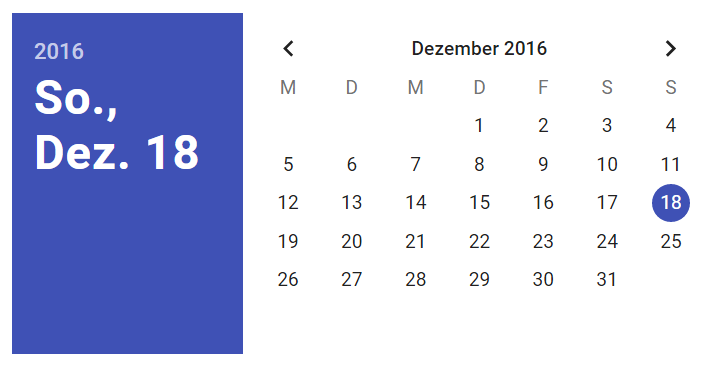
\includegraphics[width=\textwidth,height=\textheight,keepaspectratio]{datPic.png}
			\caption[Paper Date Picker]{Paper Date Picker Web Component Ansicht}
			\label{img:datPic}
		\end{figure}
		Das \emph{Web Component} ist in Abbildung \ref{img:datPic} dargestellt. Es nutzt Texte und Symbole. Die Adaptivität dieses Elements sollte durch eine mögliche Veränderung des Kontrasts, der Schrift, der Leserichtung, dadurch wiederum der Anordnung der Elemente und wenn möglich der Bereitstellung von Text- und Symbol-Alternativen ermöglicht werden.
		\newline
		Der Kontrast der Texte, also der Datenelemente, gegenüber dem Hintergrund sollte sich an den Nutzer anpassen. Diese sollten sich hochgradig voneinander unterscheiden lassen können. Auf die Schrift der Texte sollte Einfluss genommen werden können. So sollte die Schriftart und insbesondere die Schriftgröße anpassbar sein. Um sich an die Leserichtung des Nutzers anzupassen, sollte Einfluss auf die Anordnung der Texte und auch Elemente genommen werden. Zuletzt sollten, wenn möglich, Alternativen für Texte oder im Gegensatz dazu, zu Darstellungen, geboten werden.
		\subsection{Einrichtung des Paper Date Picker Web Component}
		Das \emph{Paper Date Picker Web Component} ist auf GitHub gespeichert. Es wurde wiederum ein \enquote{fork} durchgeführt um an diesem weiterarbeiten zu können und es zu erweitern. Für die Abhängigkeiten des Elements wurde wieder \emph{Bower} genutzt. Nachdem es eingebunden ist und alle Abhängigkeiten installiert sind kann das \emph{Web Component} unter dem \ac{HTML} Bezeichner \enquote{<paper-date-picker>} genutzt werden.
		\subsection{Umsetzung der Programmierung}
		Im folgenden wird die konzipierte Adaptivität des Elements im Programmcode umgesetzt. 
		\subsubsection{Text-Alternativen}
		Um Text-Alternativen für Text-Elemente zu ermöglichen muss es möglich sein diese zu ersetzen ohne ein Verlust an Informationen zu erleiden. Die Text-Komponenten dieses Elements bestehen aus Bezeichnungen für Tage, Monate, Jahre und Zahlen. Es ist nicht möglich diese durch eindeutige Symbole zu ersetzen. Deshalb können in diesem \emph{Web Component} keine Text-Alternativen angeboten werden.
		\newline
		Es ist jedoch möglich die Symbole dieses Elements zu ersetzen.
		

\chapter{Vergleich}
Kapitel über den Vergleich
	

	\printbibliography
\end{document}